\documentclass[11pt,a4paper]{article}
\usepackage{fontspec}
\setmainfont{TeX Gyre Pagella}
\newfontfamily\headfont{Inter}[UprightFont=*-ExtraBold,BoldFont=*-ExtraBold,Extension=.otf,Path=/usr/share/fonts/opentype/inter/]
\usepackage[a4paper,margin=2.3cm]{geometry}
\usepackage{graphicx,booktabs,float,caption,array,xcolor,longtable}
\usepackage[hidelinks]{hyperref}
\usepackage{titlesec}
\usepackage{setspace}
\setstretch{1.05}
\setlength{\parindent}{0pt}\setlength{\parskip}{0.55em}
\titleformat{\section}{\headfont\Large}{\thesection}{0.8em}{}
\titleformat{\subsection}{\headfont\large}{\thesubsection}{0.8em}{}
\captionsetup{font=small,labelfont=bf}
\urlstyle{same}
\hypersetup{pdftitle={England in 1086, drawn},pdfauthor={Tristan Hotham}}
\begin{document}
\begin{center}
{\Large\bfseries England in 1086, Drawn\par}
\vspace{0.4em}
{\large Turning Domesday Book's figures into a hand-inked map of every vill\par}
\vspace{1.2em}
{\large Tristan Hotham\par}
\vspace{0.3em}
{\small Independent researcher\\ ORCID: 0000-0003-4931-9349\\ DOI: \href{https://doi.org/10.5281/zenodo.24045206}{10.5281/zenodo.24045206}\par}
\vspace{0.8em}
2026
\end{center}
\begin{quote}\small
\begin{center}\textbf{Abstract}\end{center}
Domesday Book records, for most of England in 1086, how many households each vill had, its plough teams, mills, churches, woodland, fisheries, salt-pans and, in some counties, its livestock. I draw those records as a zoomable map in the style of a hand-inked fantasy map, in which nothing modern appears and every mark stands for something the survey counted. Using the Hull Domesday Project's coded database, I place one dwelling for each of the 273,961.5 households counted (260,042 at the 13,068 located places), one water wheel for each mill on the nearest stream (5,408 drawn), 71,419 plough teams of eight oxen and 27,154 drawings of flocks, herds and hives over each vill's lands, and woods where the survey measures woodland. The boroughs are drawn from the houses each borough entry counts, including the empty and destroyed ones. This methods note sets out how each glyph is derived, the thresholds and conventions used, and what Domesday does not record. The map shows how sparsely England was settled: the median vill counted 16 households, 66.2\% had fewer than 25, and only 257 are drawn with a hundred dwellings or more.

\textbf{Keywords:} Domesday Book; 1086; historical GIS; settlement; mills; cartography; fantasy map; visualisation
\end{quote}

\section{Introduction}
Domesday Book is the most complete account of a medieval kingdom that survives. In 1086 the King's commissioners asked, of every manor, who held it in 1066 and who held it now, how many hides it paid tax on, how many ploughs and people it had, its mills, meadow, woodland, pasture, fisheries and salt-pans, and what it was worth then and now \cite{darby}. Historians have long turned those answers into maps of densities and distributions. This study does something more literal: it draws each vill as the survey describes it, on a map in the manner of the inked maps in the front of fantasy novels, so that a reader can zoom from the whole kingdom to a single village and see what Domesday says was there.

The map is built on my earlier Inked World engine \cite{inkmap}, which draws mountains from elevation, coasts, rivers and lettering in one hand-drawn style. For 1086 every modern layer is removed and replaced with drawings derived from Domesday. The page is at \url{https://maps.tristanhotham.com/domesday-world/}. This note documents the rules behind each mark so that the picture can be read critically: what is counted, what is estimated and what is decoration.

\section{Data}
\textbf{Domesday.} The Hull Domesday Project's coded database of Great Domesday and its transcription of the Phillimore translation (Professor J.J.N. Palmer, George Slater and the University of Hull), as packaged entry by entry in the realm-domesday repository \cite{realm}. It holds 22,571 entries, of which 20,438 describe a place, and 14,334 places, of which 13,068 are located to a 1 km grid square. Little Domesday (Essex, Norfolk and Suffolk) is parsed from the translation. Each entry carries households by class, plough teams, ploughlands, mills, meadow, woodland measured in pigs, fisheries, salt-houses, livestock, values in 1066 and 1086, a church, castle, market or waste flag, and the people who held it before and after the Conquest. Hull's transcription omits Yorkshire's text, so its coded figures are used but nothing is read from its words. The data are licensed CC BY-NC-SA, and so are the files derived from them here.

\textbf{Companion studies.} The allocation of figures follows my Domesday Destiny study \cite{destiny}; mill totals agree with the Domesday mills study \cite{mills}, waste entries with the Harrying of the North study \cite{harrying} and the castles named with the Norman castles study \cite{castles}.

\textbf{Other sources.} Religious houses founded by 1086 come from the English Monastic Archives database (UCL) and markets recorded by 1086 from the Gazetteer of Markets and Fairs in England and Wales to 1516 \cite{markets}, both from the Mind Your Manors data set; Roman roads from Itiner-e \cite{itinere}; castles dated to 1086 or before but not named in Domesday from Wikidata through the Norman castles study. Water areas and stream lines come from OpenStreetMap through OpenFreeMap's vector tiles \cite{osm}, used only to keep drawings off the water and to place mills; elevation from the AWS Terrain Tiles \cite{terrain}.

\section{Methods}
\subsection{From entries to vills}
An entry's figures are given to the places it describes, shared equally when it describes several \cite{destiny}; this gives 273,961.5 households, the same total as the companion study. For the drawing only, an entry that also names located dependent members (outliers or sokeland) spreads its households and resources over the head and the members, the head taking a double share, so that a great manor such as Leominster is not drawn as one town of several hundred houses. Members that are boroughs take no share of a rural manor's people (an entry that owns houses in London does not move its villagers there), and salt-houses held in the inland wiches are moved to the wich.

\subsection{Dwellings}
Domesday counts heads of household: villagers, smallholders, cottagers, slaves, freemen and free men, priests, burgesses and others. A household is roughly a family, so each is drawn as one dwelling, rounded half up. Each vill is given a simple plan. Plots are laid every 80 m (105 m in a hamlet of fewer than six, 55 m or less in a borough) along both sides of the streets and lanes of today's OpenStreetMap within 650 m of the vill's point (1.6 km in a borough), used as a proxy for the old village street, and filled nearest the centre first, so the core is dense and the edges thin; only plots nearer to this vill than to any other are used. Where today's lanes give too few plots, the vill gets a lane of its own through its centre (a cross lane in vills of more than 40 households) or, in a share of vills of 8 to 40 households, a green with houses round it (10,537 vills on streets, 1,620 on a lane of their own, 338 round a green). The church and the lord's hall stand at the core. Each plot is tested against the water areas of OpenStreetMap at zoom 13 (256 pixels to a tile, about 19 m); 74 dwellings could not be placed. The drawing of each follows the classes counted: longhouses for villagers and freemen, cottages for smallholders, cottagers, slaves and priests, town houses for burgesses. The map thins them with the zoom in proportion: one drawing per household from zoom 12, one for every two at zoom 11, and further out a single glyph per vill with one to six huts by its size (under 5, 5 to 9, 10 to 19, 20 to 39, 40 to 79 and 80 or more households).

\subsection{Boroughs}
Domesday describes the boroughs in their own terms: houses, messuages, sites and burgesses, with counts before 1066 and in 1086 and of houses empty or destroyed. For 73 boroughs I take the dwellings from those counts, by hand for the largest and as the sum of the 1086 counts for the rest, and draw the empty and destroyed ones roofless (3,191 in all). Table~\ref{tab:towns} lists the largest. Lincoln, for example, had ``970 inhabited messuages before 1066'', of which ``166 were destroyed because of the castle'' and ``760 are now inhabited''. York's text is not in the transcription, so it is drawn from an estimate of 540 inhabited and 540 empty dwellings, and the popup says so. London and Winchester were left out of the survey; their houses are estimated (Section~\ref{sec:est}). Where OpenStreetMap maps a city wall within 1.5 km of a borough (the Roman walls of London, York, Lincoln, Chester, Colchester, Canterbury, Winchester and Exeter, and later medieval circuits that mostly follow them), that wall is drawn and its outline becomes the walled core: houses fill the streets inside it first, densest at the centre, before spilling along the roads outside (12 boroughs). The walls are those mapped today, so some stretches are later than 1086.

\subsection{Estimates for places without a usable figure}\label{sec:est}
Some places Domesday names give no usable household figure: an entry with land, ploughs or a value but no people, a vill called waste with nobody counted, and the two great towns left out of the survey. Drawn literally they would be empty. They are instead given estimated dwellings, drawn visibly paler (dotted outlines; roofless for waste), flagged in the popup with the method, listed in \texttt{data/estimates.csv}, and kept out of every recorded total in this paper. The method is deliberately conservative. For a place with no households, the first available of its plough teams, ploughlands, value in 1086, value in 1066 and hides or carucates is multiplied by the county median of households per unit of that measure among vills with both (all England where a county has fewer than ten); for a waste vill, only measures that describe it before or apart from its wasting (value in 1066, ploughlands, hides or carucates). The result is capped at the median households of the vills of its hundred (231 capped), with at least one dwelling. Where no measure is given, the lower quartile of the hundred's vills is used (125 places; 1,051 by a ratio). For London and Winchester I take the low end of historians' estimates of their people around 1100, about 10,000 for London \cite{brooke,keene} and 5,000 for Winchester \cite{biddle}, at 4.5 people a household (Darby used 4 to 5), giving 2,222 and 1,111 dwellings. In all 9,237 dwellings are estimated at 1,178 places: 3,369 at 645 places with no usable figure, 2,535 empty ones at 531 waste vills, and 3,333 in the two towns. Nothing is estimated for lands the survey did not cover.

\begin{table}[H]\centering\small
\caption{The largest places as drawn (dwellings, including borough estimates).}\label{tab:towns}
\begin{tabular}{llr}\toprule Place & County & Dwellings drawn \\ \midrule
Norwich & NFK & 1,145 \\
Lincoln & LIN & 760 \\
Thetford & NFK & 720 \\
York & YKS & 540 \\
Milton Regis & KEN & 425 \\
Wymondham & NFK & 396 \\
Folkestone & KEN & 395 \\
Leicester & LEC & 371 \\
Aldington & KEN & 343 \\
Sandwich & KEN & 339 \\
\bottomrule\end{tabular}\end{table}

\subsection{What each glyph means}
Table~\ref{tab:glyphs} lists every drawing and the rule behind it. Two principles hold throughout: a glyph stands for something the survey records at that vill, and the number of glyphs follows the number recorded, at a stated rate where one drawing per item would be unreadable.

\begin{table}[H]\centering\footnotesize
\caption{The glyphs and their rules.}\label{tab:glyphs}
\begin{tabular}{p{4.2cm}p{7.8cm}p{2.6cm}}\toprule Glyph & Rule & Coverage \\ \midrule

Dwelling (longhouse, cottage, burgess's house) & one per household counted, rounded half up; the kind follows the classes the entry counts & every vill \\
Empty or wasted dwelling & the borough's own count of waste or empty houses & 73 boroughs \\
Lord's hall & three households or more, and demesne ploughs or a value of \pounds 2 or more & rural vills \\
Church; stone church; minster; cathedral & an entry mentions a church; 40 or more dwellings or a borough; canons, monks or a minster named; the see of 1086 & every vill \\
Watermill & one per mill, fractions rounded half up, on the nearest stream or river within 1.5 km & every vill \\
Fishery (eel weir) & a fishery or eels recorded; nearest stream within 2 km, or shore within 3 km & non-Yorkshire text and fields \\
Salt-pans; brine pits & salt-houses recorded, one hearth per three; nearest shore within 6 km, or the inland wiches & every vill \\
Vineyard; park; hedged enclosure & named in the text & non-Yorkshire text \\
Plough team & one per team (eight oxen) & every vill \\
Sheep; pigs; cattle; goats & one per 20; 10; 5; 10 & where counted \\
Cobs and horses; wild mares; beehives; oxen & one per 3; 5; 5; 4 & where counted \\
Swine at pannage & one per 50 pigs of woodland & where woodland is measured in pigs \\
Woodland & 1 ha a pig; length $\times$ breadth $\times$ 0.7; 0.4 ha an acre & where woodland is measured \\
Castle & named in Domesday, or dated to 1086 or before (marked) & 41 named \\
Religious house & founded by 1086 in the English Monastic Archives & 103 \\
Market & recorded in Domesday or by 1086 in the Gazetteer & every vill \\
Town wall & the line of the city walls in OpenStreetMap (Roman and medieval) within 1.5 km of a borough & 12 towns \\
Estimated dwelling (pale, dotted) & no usable household figure: see Section~\ref{sec:est}; not in any total & 645 vills \\
Estimated empty dwelling (pale, roofless) & a waste vill with nobody counted: see Section~\ref{sec:est} & 531 vills \\
Open fields; meadow & ridge and furrow round the village, 48 ha a plough team; Domesday's meadow acres by the stream & every vill \\
\bottomrule\end{tabular}\end{table}

\begin{figure}[H]\centering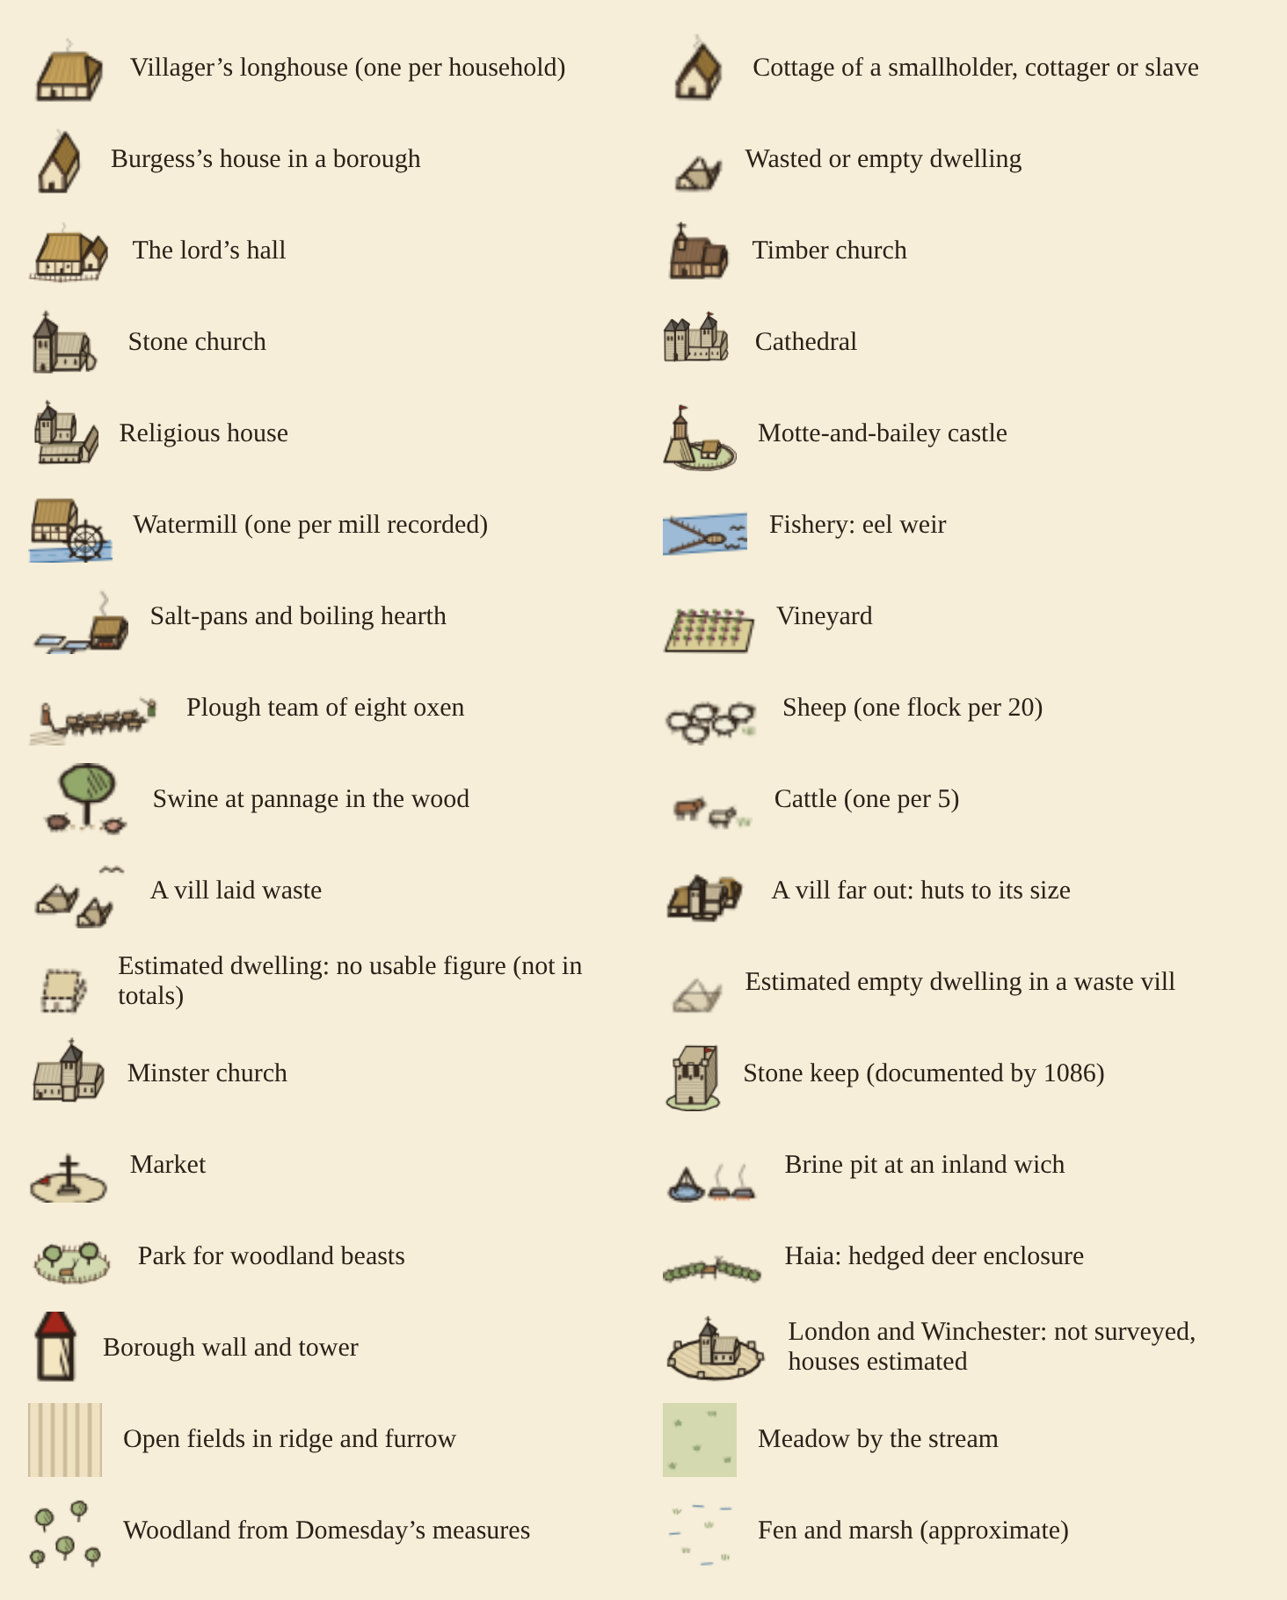
\includegraphics[width=0.92\textwidth]{legend2.png}\caption{The period drawings, in the Inked World's pen.}\end{figure}

\subsection{Mills and water}
No source says where on its land each mill stood, but a watermill needs moving water. Each mill is therefore set on the nearest stream or river line in today's OpenStreetMap within 1.5 km of its vill, at points 110 m apart along the water, with the mill house on the village side of the wheel. Domesday counts 6,073.8 mills at located places, with many halves and thirds shared between manors; rounding each place's total half up gives 5,679, of which 5,408 (95.2\%) have a stream within 1.5 km and are drawn. The other 271 are listed in the popup but not drawn: a mill on dry land would be a worse error than a missing wheel. Fisheries go on the nearest stream within 2 km or the nearest shore within 3 km; coastal salt-pans on the nearest shore within 6 km; the brine pits and hearths of Droitwich and the Cheshire wiches round the town itself.

\subsection{The vill's lands}
Round the houses lie the open fields, drawn as ridge and furrow in two or three great fields with the strips running different ways, at 48 ha (about 120 acres) a plough team (half the ploughlands where no teams are counted), up to 60\% of the vill's land: 2,396,200 ha in all. Meadow is laid by the nearest stream at 0.4 ha a Domesday acre (58,208 ha), and woodland further out. Plough teams are drawn only in their own vill's fields, or within 700 m of its houses where no field is drawn. Flocks and herds are scattered over the vill's own lands: points nearer to it than to any other located vill (a Voronoi cell), within 2.6 km, dry, outside the drawn houses and at least 60 m apart. Flocks and wild mares furthest out, pigs, cattle and hives at the village edge, swine at pannage inside the woods. The rates are one drawing per plough team, per 20 sheep, 10 pigs, 5 cattle, 10 goats, 3 cobs or horses, 5 wild mares, 5 beehives and 4 oxen counted apart from the teams, and at least one where any are recorded. Domesday counts livestock almost only in Little Domesday and the Exeter Domesday counties; elsewhere the absence of flocks is an absence of counting.

\subsection{Woodland, marsh and the lands beyond}
Domesday measures woodland in pigs (the swine it could feed), in leagues and furlongs, or in acres. These measures do not convert reliably to area \cite{darby}, so I use drawing conventions: one hectare a pig; length times breadth times 0.7 for linear measures (a league taken as 12 furlongs, about 2.4 km; one dimension alone as a strip a quarter as wide); 0.4 ha an acre; and 10 ha where woodland is named without a measure. The wood is laid on a 150 m grid on the far side of the vill's lands, up to 70\% of them. The marshes are drawn where the ground lies below a set height inside five basins on today's elevation (Terrarium tiles at zoom 8): the Fens (3.5 m), the Somerset Levels (7 m), the Humberhead Levels (5 m), Romney Marsh and the Pevensey Levels (4 m). The Wantsum Channel, which made Thanet an island, is drawn by hand; the New Forest's outline joins the 45 vills the Hampshire folios list in it. Britain more than about 15 km from any located vill and joined to the north, Wales or Man is washed paler and lettered as not surveyed: 48.8\% of Great Britain and 8.7\% of today's England.

\subsection{Removing the modern}
The engine's modern layers are removed: roads, railways, buildings, modern names, modern woods and fields, airports, heritage, ships and flying machines. Canals and drains, the straight cuts of the Fens by their names, and inside the fens and levels every waterway except the old rivers by name (so the Nene's straight channel below Peterborough, the Bedford rivers and the Dutch River go) are left out. Roman roads are drawn as single dashed tracks, so they cannot be mistaken for railways. Ponds and lakes are left out entirely, since in lowland England nearly all are modern pits, ponds and reservoirs and the tiles cannot tell them from the few natural meres. Coasts, rivers and relief remain those of today. Roman roads, still the country's main roads in 1086, come from Itiner-e, and the four great highways are lettered along approximate lines. Shire edges are approximate (the Voronoi cells of each shire's vills) and 692 hundreds and wapentakes are lettered at the median of their vills.

\section{Results}
The map draws 260,042 dwellings at 11,318 vills (Figure~\ref{fig:eng}). Settlement was thin: 31.4\% of vills with people counted fewer than ten households and the median counted 16 (Figure~\ref{fig:sizes}). The largest places as drawn are Norwich (1,145 dwellings), Lincoln (760), Thetford (720) and York (540, an estimate), and several great manors whose households were spread over many hamlets (Table~\ref{tab:towns}).

\begin{figure}[H]\centering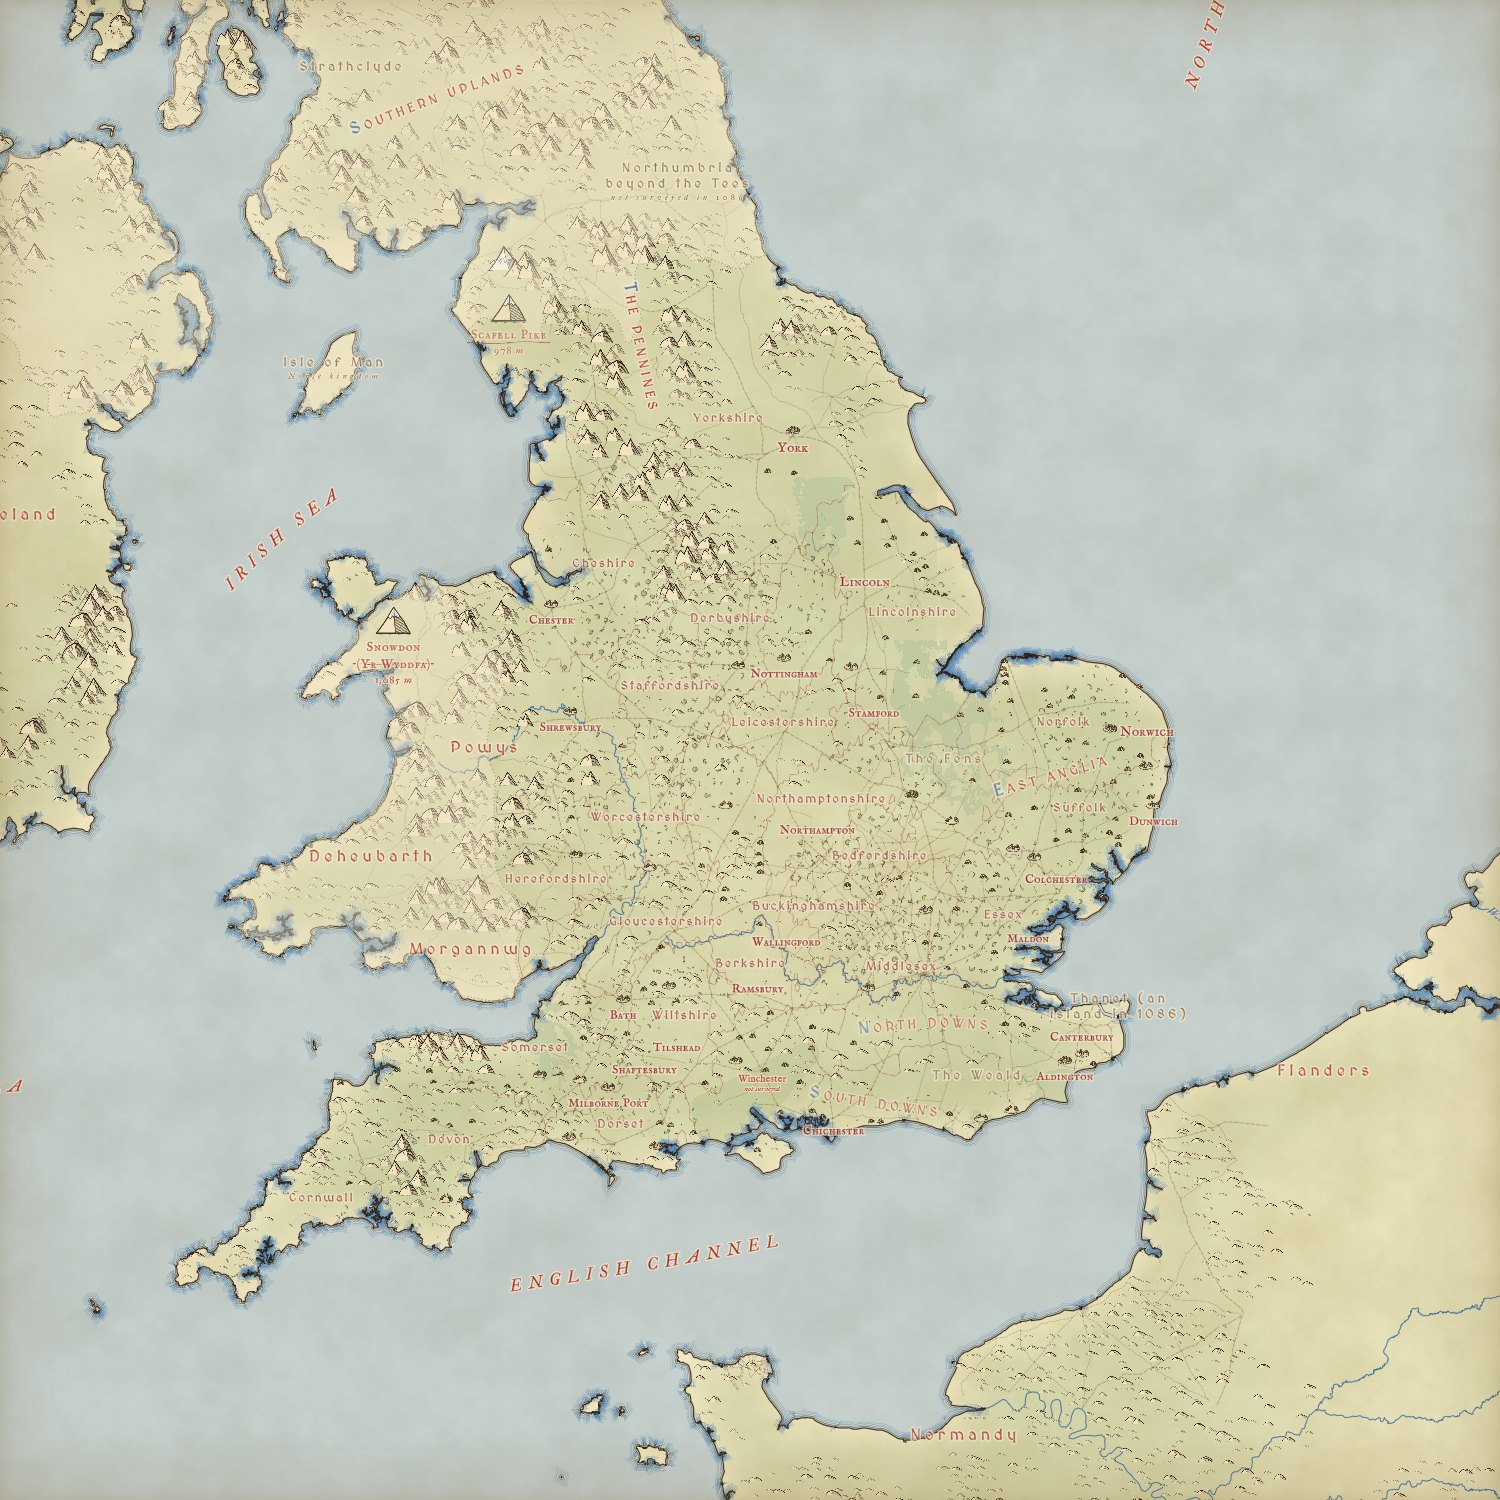
\includegraphics[width=0.78\textwidth]{b_england.jpg}\caption{England in 1086 at the scale of the kingdom: a glyph per vill, sized to its households, with Domesday's woods, the marshes and the Roman roads.}\label{fig:eng}\end{figure}
\begin{figure}[H]\centering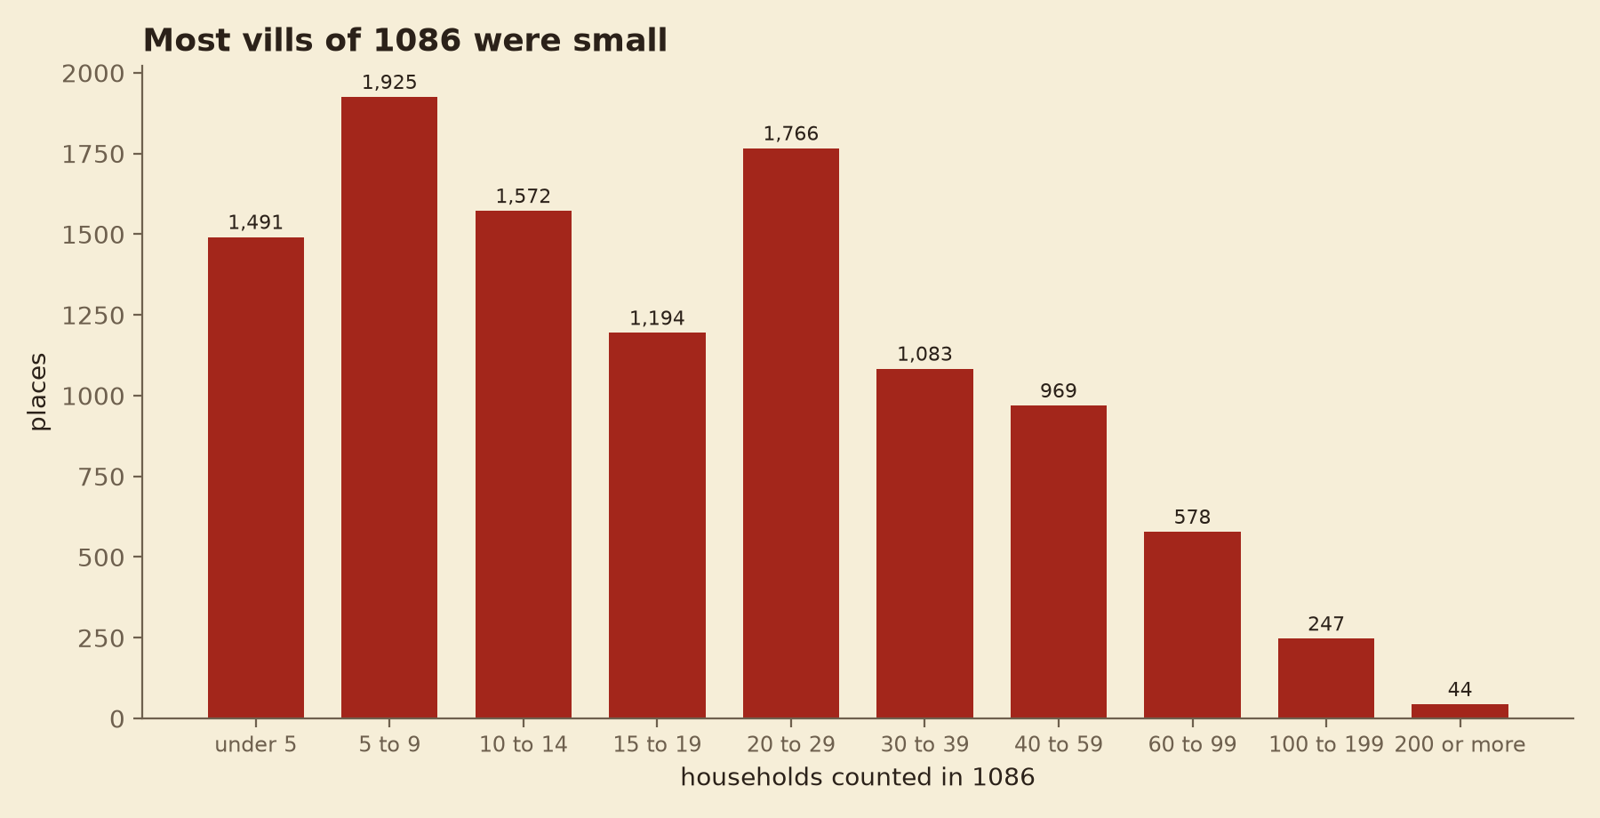
\includegraphics[width=0.85\textwidth]{b_sizes.png}\caption{Places by the households Domesday counts.}\label{fig:sizes}\end{figure}

The working countryside dominates once one zooms in: 71,419 plough teams (Domesday counts 77,513.5, so about 620,108 oxen), 5,408 mills turning on their streams (Figure~\ref{fig:mills}), 2,784 churches, 868 eel weirs and 527 salt hearths. Churches are recorded at 25.7\% of vills with people and mills at 33.1\%. Livestock are drawn where counted, which is mostly East Anglia and the south-west: Little Domesday holds 49.1\% of the 252,644 sheep the survey records (Figure~\ref{fig:suffolk}). Woodland is drawn over about 4,378 square kilometres.

\begin{figure}[H]\centering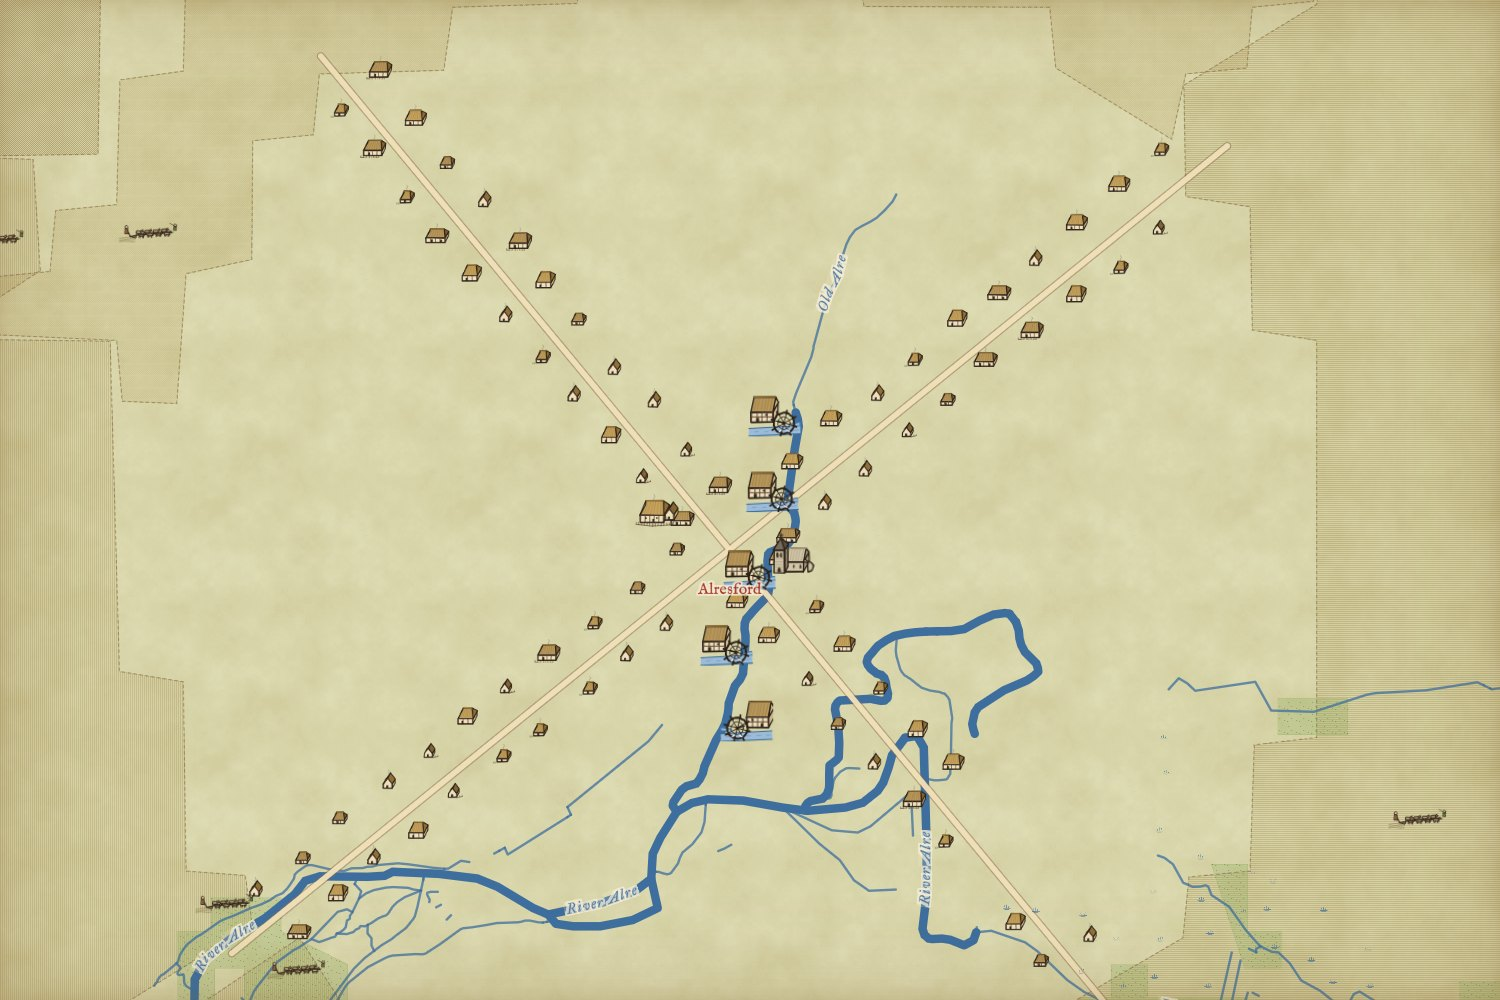
\includegraphics[width=0.92\textwidth]{b_mills.jpg}\caption{Alresford, Hampshire: mills set on the River Alre, the village's houses one per household.}\label{fig:mills}\end{figure}
\begin{figure}[H]\centering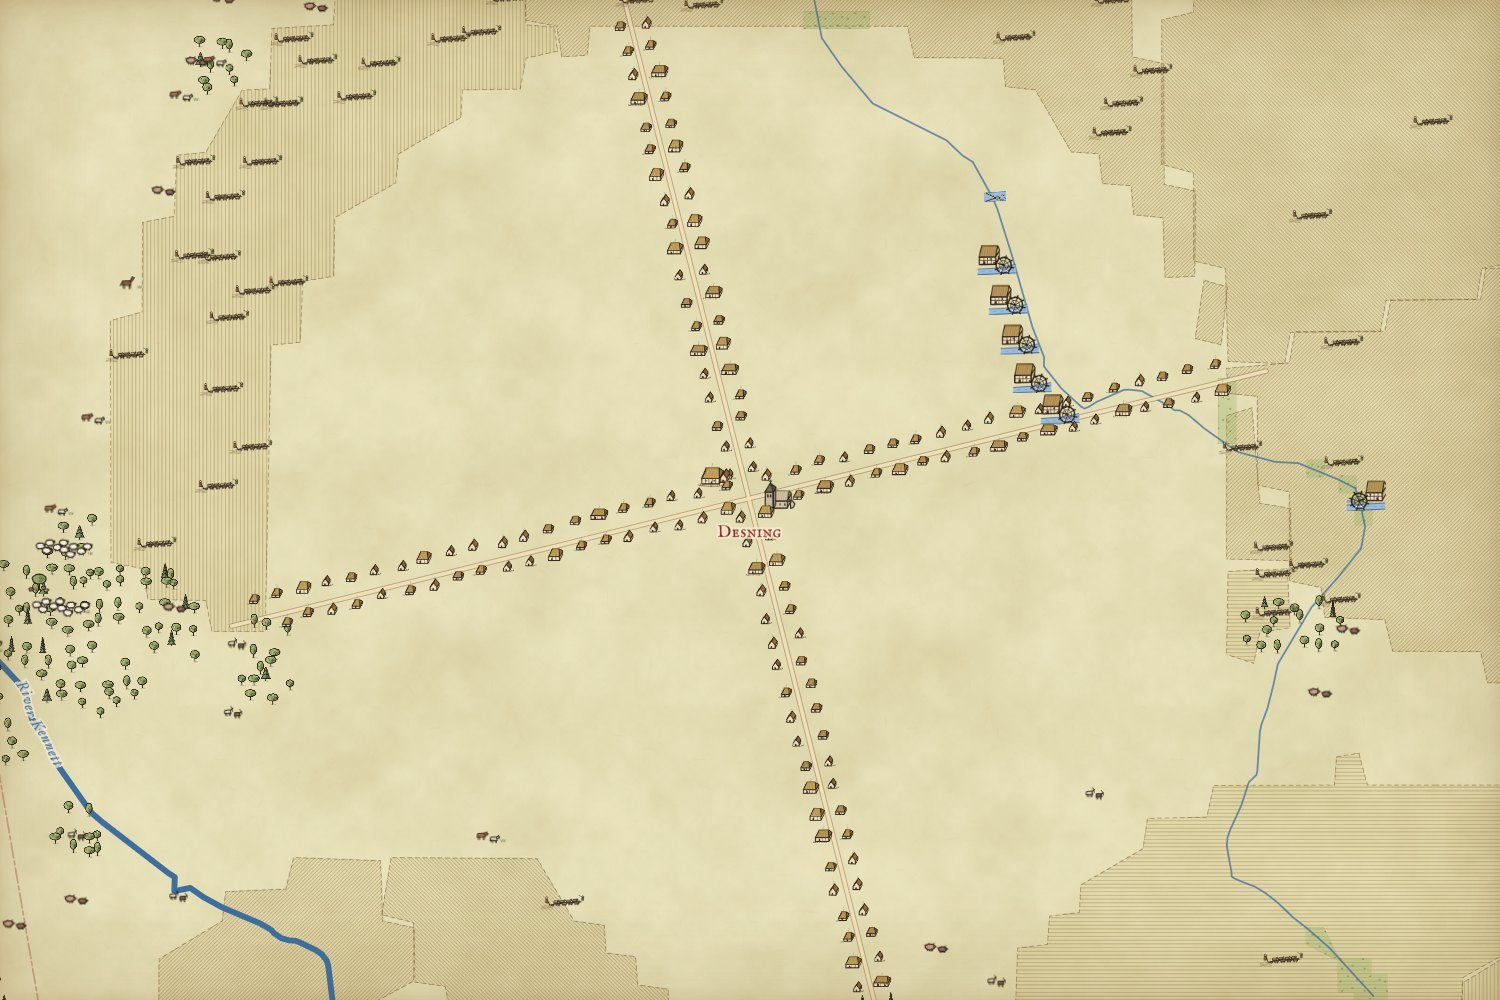
\includegraphics[width=0.92\textwidth]{b_suffolk.jpg}\caption{Desning, Suffolk: a large vill with five mills, plough teams, flocks and herds over its lands.}\label{fig:suffolk}\end{figure}

The towns carry the scars of the Conquest (Figure~\ref{fig:york}). 1,345 entries call land waste, 520 of them in Yorkshire, after the Harrying of the North of 1069 to 1070; 567 vills with nobody counted are drawn as burnt and roofless huddles.

\begin{figure}[H]\centering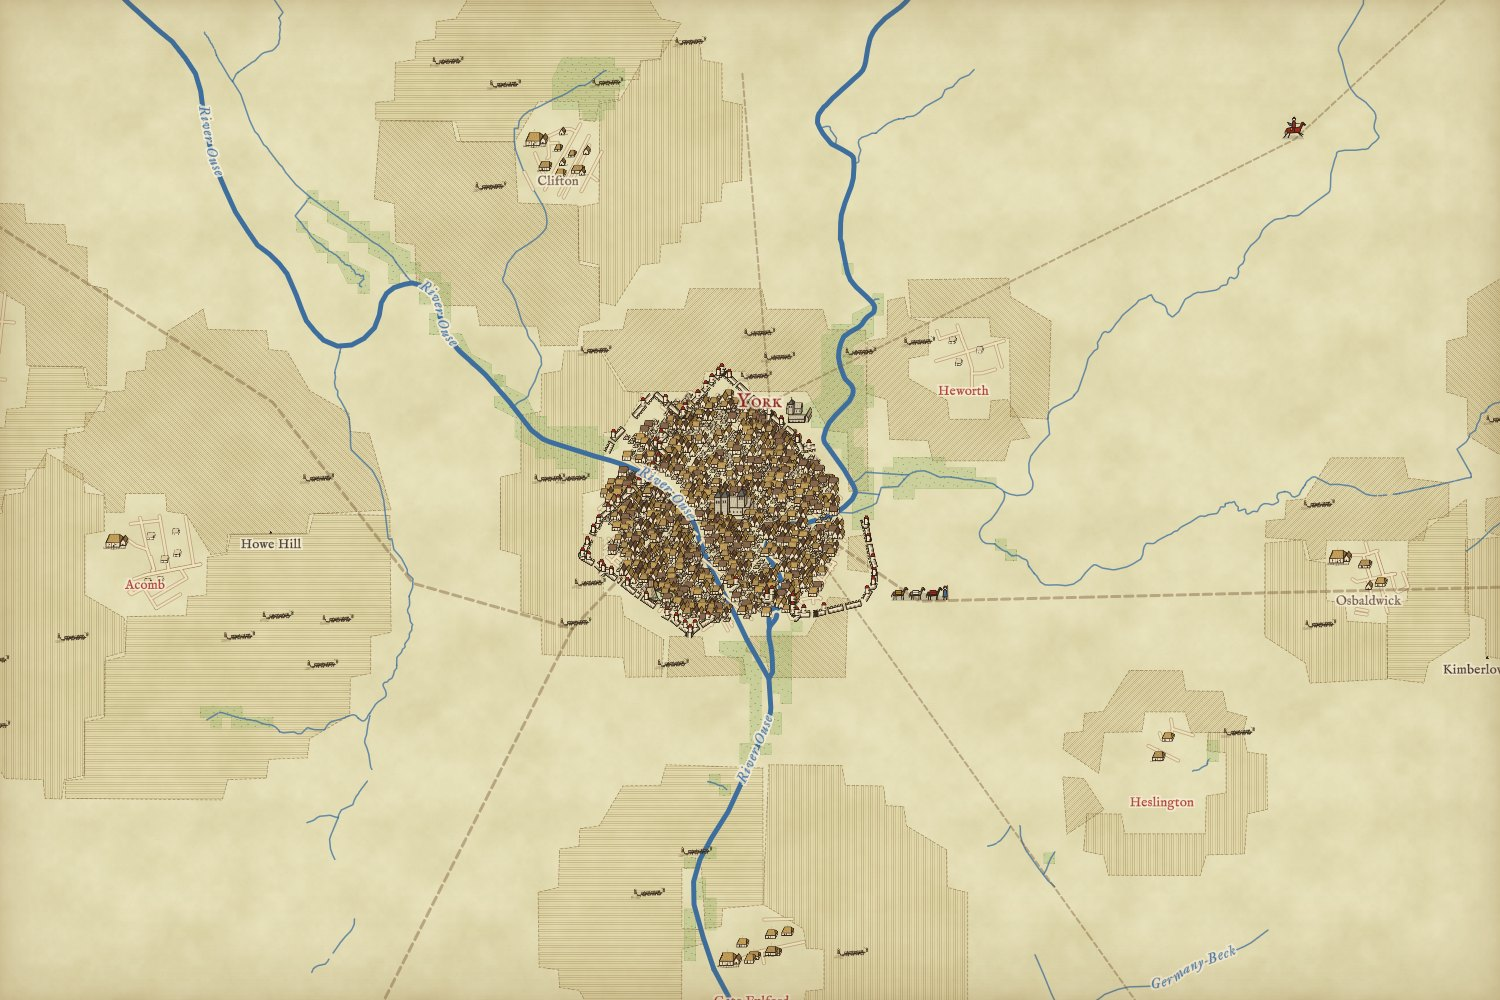
\includegraphics[width=0.92\textwidth]{b_york.jpg}\caption{York, drawn from an estimate of 540 inhabited and 540 empty dwellings, packed along its streets inside the line of its walls, with minster, castle and abbey.}\label{fig:york}\end{figure}
\begin{figure}[H]\centering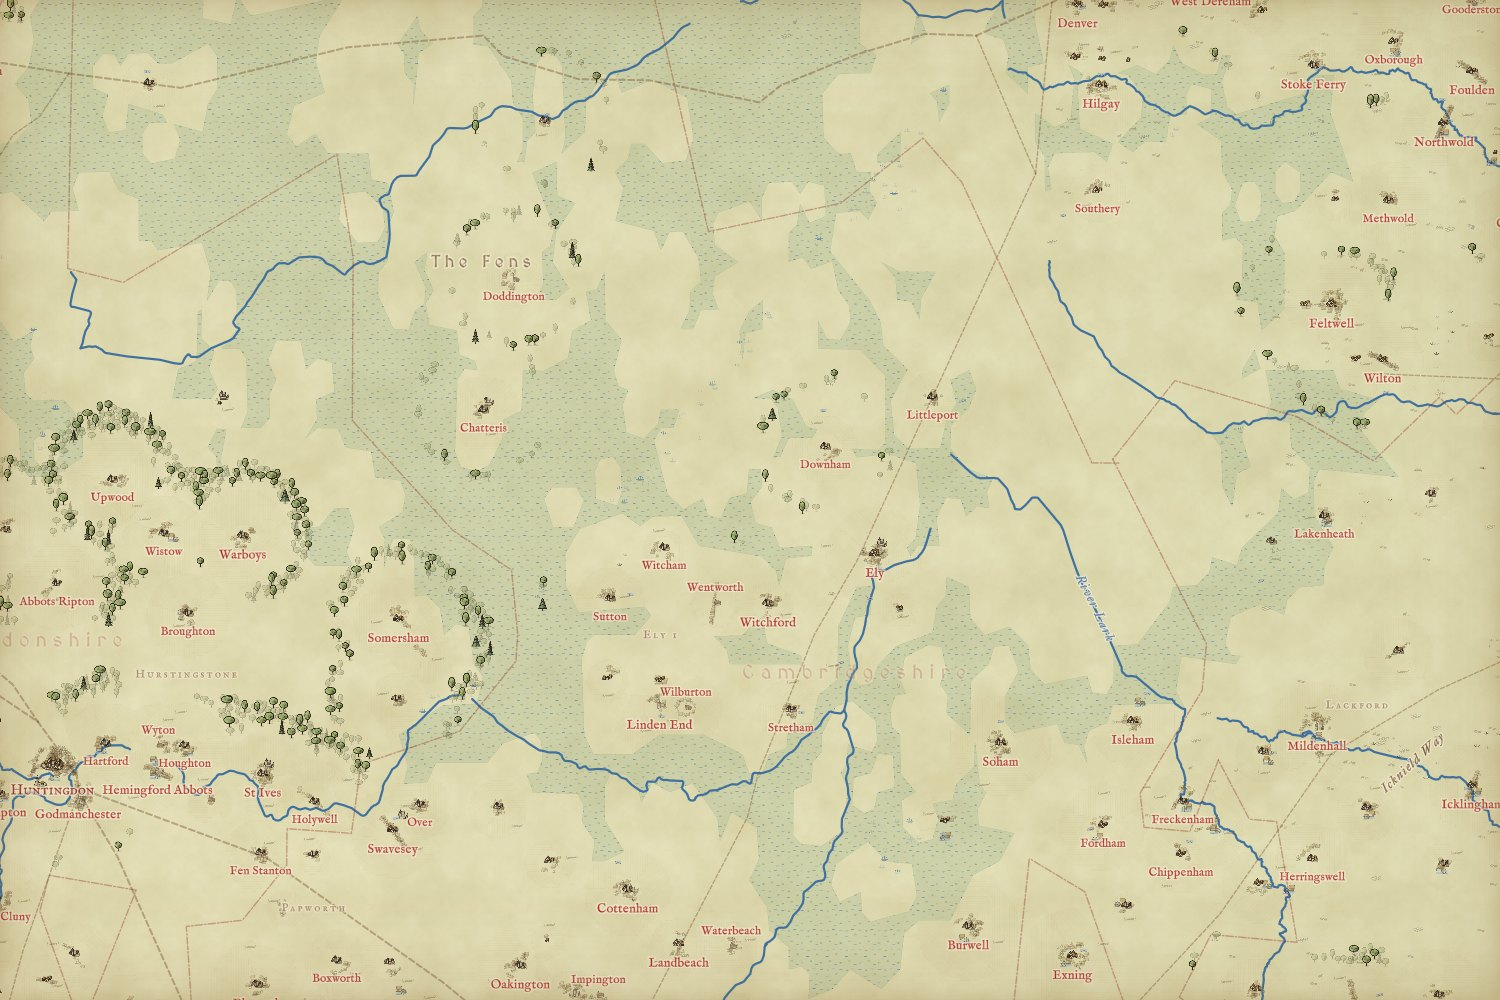
\includegraphics[width=0.92\textwidth]{b_fens.jpg}\caption{The Fens and Ely: marsh drawn from low ground, vills on the fen islands and edges.}\end{figure}

\section{Limitations}
Domesday counts households, not people, and omits many: lords' households, many priests, and townsfolk not liable to dues. It also leaves out the north beyond the Tees and the Ribble, most of Wales, London and Winchester. Hull located 13,068 of 14,334 places, each at the centre of a 1 km square. The allocation shares an entry's figures equally among the places it describes, and the drawing spreads them over named members; both are conventions. The borough estimates rest on Domesday's own counts but those counts mix houses, messuages and burgesses. The estimated dwellings (Section~\ref{sec:est}) are conventions to avoid drawing named places empty, not findings. Today's streets and walls stand in for the plans of 1086. Woodland, marsh, the town walls, the shire edges and the New Forest are approximate drawing devices; the mill, fishery and salt positions are plausible, not known. Today's rivers and coasts stand in for those of 1086, and some Fen channels and lakes are later. Travellers on the roads are decoration. The map is a picture of the record, to be read with its popups, not a reconstruction of the landscape.

\section{Data availability}
The map, code and data are at \url{https://github.com/Tristan-Hotham/domesday-world} and archived with this paper at \href{https://doi.org/10.5281/zenodo.24045206}{10.5281/zenodo.24045206}. Code is MIT; the files derived from the Hull Domesday data are CC BY-NC-SA 4.0; other text and figures CC BY 4.0. Map renders contain OpenStreetMap data (ODbL).

\section*{AI assistance}
I wrote the text, with drafting and editing assistance from Claude (Anthropic), which also helped prepare the analysis code. I reviewed and checked all text and results.

\begin{thebibliography}{99}
\bibitem[Biddle(1976)]{biddle} Biddle, M. (ed.) (1976) \emph{Winchester in the Early Middle Ages: an edition and discussion of the Winton Domesday}. Winchester Studies 1. Oxford: Clarendon Press.
\bibitem[Brooke and Keir(1975)]{brooke} Brooke, C. N. L. and Keir, G. (1975) \emph{London 800 to 1216: the shaping of a city}. London: Secker and Warburg.
\bibitem[Keene(2000)]{keene} Keene, D. (2000) London from the post-Roman period to 1300. In D. M. Palliser (ed.) \emph{The Cambridge Urban History of Britain, vol. 1}. Cambridge: Cambridge University Press.
\bibitem[Darby(1977)]{darby} Darby, H. C. (1977) \emph{Domesday England}. Cambridge: Cambridge University Press.
\bibitem[Palmer et al.]{hull} Palmer, J. J. N., Slater, G. and the University of Hull. Hull Domesday Project database and Domesday Explorer. \url{https://digitalcollections.hull.ac.uk/collections/3t945r28b} (CC BY-NC-SA).
\bibitem[Embabel Worlds(2026)]{realm} realm-domesday: Domesday Book as a graph. \url{https://github.com/embabel-worlds/realm-domesday}.
\bibitem[Hotham(2026a)]{inkmap} Hotham, T. (2026) The Inked World. Zenodo. \url{https://doi.org/10.5281/zenodo.23860253}.
\bibitem[Hotham(2026b)]{destiny} Hotham, T. (2026) Domesday Destiny. \url{https://maps.tristanhotham.com/domesday-destiny/}.
\bibitem[Hotham(2026c)]{mills} Hotham, T. (2026) Domesday mills. \url{https://maps.tristanhotham.com/domesday-mills/}.
\bibitem[Hotham(2026d)]{harrying} Hotham, T. (2026) The Harrying of the North. \url{https://maps.tristanhotham.com/harrying-of-the-north/}.
\bibitem[Hotham(2026e)]{castles} Hotham, T. (2026) Norman castles. \url{https://maps.tristanhotham.com/norman-castles/}.
\bibitem[Letters et al.]{markets} Letters, S. et al. Gazetteer of Markets and Fairs in England and Wales to 1516. Centre for Metropolitan History; and the English Monastic Archives database, UCL; via the Mind Your Manors data set.
\bibitem[de Soto et al.(2025)]{itinere} de Soto, P. et al. (2025) Itiner-e: the digital atlas of ancient roads. CC BY 4.0.
\bibitem[OpenStreetMap]{osm} OpenStreetMap contributors, via OpenFreeMap (OpenMapTiles schema). ODbL 1.0.
\bibitem[Mapzen]{terrain} AWS Terrain Tiles (Terrarium). \url{https://registry.opendata.aws/terrain-tiles/}.
\end{thebibliography}
\end{document}
